%\documentclass[11pt,handout]{beamer}
\documentclass[9pt]{beamer}
\usetheme[white]{Illinois}

\title[]{Hydrogen Economy in Champaign-Urbana, IL}
\subtitle[]{ANS Annual meeting 2020}
\author[]{Roberto Fairhurst Agosta}
\date[05.12.2020]{June 10, 2020}
\institute[UIUC]{University of Illinois at Urbana-Champaign}

%\usepackage{bbding}
\usepackage{amsfonts}
\usepackage{amsmath}
\usepackage{xspace}
\usepackage{graphicx}
\usepackage{subfigure}
\usepackage{booktabs} % nice rules for tables
\usepackage{microtype} % if using PDF
\usepackage{bigints}
\usepackage{minted}
\usepackage[absolute,overlay]{textpos}
\usepackage{tikz}
\usetikzlibrary{positioning, arrows, decorations, shapes}
\usetikzlibrary{shapes.geometric,arrows}
\definecolor{illiniblue}{HTML}{B1C6E2}
\tikzstyle{bblock} = [rectangle, draw, fill=illiniblue,
text width=10em, text centered, rounded corners, minimum height=4em]
\tikzstyle{sbblock} = [rectangle, draw, fill=illiniblue,
text width=7em, text centered, rounded corners, minimum height=4em]
\tikzstyle{arrow} = [thick,->,>=stealth]

\newcommand{\units}[1] {\:\text{#1}}%
\newcommand{\SN}{S$_N$}%{S$_\text{N}$}%{$S_N$}%
\DeclareMathOperator{\erf}{erf}
\DeclareMathOperator{\erfc}{erfc}
\setbeamertemplate{bibliography item}[text]

%%%% Acronym support
\usepackage[acronym,toc]{glossaries}
\newacronym[longplural={metric tons of heavy metal}]{MTHM}{MTHM}{metric ton of heavy metal}
\newacronym{ABM}{ABM}{agent-based modeling}
\newacronym{ACDIS}{ACDIS}{Program in Arms Control \& Domestic and International Security}
\newacronym{AHTR}{AHTR}{Advanced High Temperature Reactor}
\newacronym{ANDRA}{ANDRA}{Agence Nationale pour la gestion des D\'echets RAdioactifs, the French National Agency for Radioactive Waste Management}
\newacronym{APP}{APP}{Abbott Power Plant}
\newacronym{ANL}{ANL}{Argonne National Laboratory}
\newacronym{API}{API}{application programming interface}
\newacronym{ARCH}{ARCH}{autoregressive conditional heteroskedastic}
\newacronym{ARE}{ARE}{Aircraft Reactor Experiment}
\newacronym{ARFC}{ARFC}{Advanced Reactors and Fuel Cycles}
\newacronym{ARMA}{ARMA}{autoregressive moving average}
\newacronym{ASME}{ASME}{American Society of Mechanical Engineers}
\newacronym{ATWS}{ATWS}{Anticipated Transient Without Scram}
\newacronym{BDBE}{BDBE}{Beyond Design Basis Event}
\newacronym{BIDS}{BIDS}{Berkeley Institute for Data Science}
\newacronym{BOL}{BOL}{Beginning-of-Life}
\newacronym{BSD}{BSD}{Berkeley Software Distribution}
\newacronym{CAFCA}{CAFCA}{ Code for Advanced Fuel Cycles Assessment }
\newacronym{CASL}{CASL}{Consortium for Advanced Simulation of Light Water Reactors}
\newacronym{CDTN}{CDTN}{Centro de Desenvolvimento da Tecnologia Nuclear}
\newacronym{CEA}{CEA}{Commissariat \`a l'\'Energie Atomique et aux \'Energies Alternatives}
\newacronym{CI}{CI}{continuous integration}
\newacronym{CNEC}{CNEC}{Consortium for Nonproliferation Enabling Capabilities}
\newacronym{CNEN}{CNEN}{Comiss\~{a}o Nacional de Energia Nuclear}
\newacronym{CNERG}{CNERG}{Computational Nuclear Engineering Research Group}
\newacronym{COSI}{COSI}{Commelini-Sicard}
\newacronym{COTS}{COTS}{commercial, off-the-shelf}
\newacronym{CSNF}{CSNF}{commercial spent nuclear fuel}
\newacronym{CTAH}{CTAHs}{Coiled Tube Air Heaters}
\newacronym{CUBIT}{CUBIT}{CUBIT Geometry and Mesh Generation Toolkit}
\newacronym{CURIE}{CURIE}{Centralized Used Fuel Resource for Information Exchange}
\newacronym{DAG}{DAG}{directed acyclic graph}
\newacronym{DANESS}{DANESS}{Dynamic Analysis of Nuclear Energy System Strategies}
\newacronym{DBE}{DBE}{Design Basis Event}
\newacronym{DESAE}{DESAE}{Dynamic Analysis of Nuclear Energy Systems Strategies}
\newacronym{DHS}{DHS}{Department of Homeland Security}
\newacronym{DOE}{DOE}{Department of Energy}
\newacronym{DRACS}{DRACS}{Direct Reactor Auxiliary Cooling System}
\newacronym{DRE}{DRE}{dynamic resource exchange}
\newacronym{DSNF}{DSNF}{DOE spent nuclear fuel}
\newacronym{DYMOND}{DYMOND}{Dynamic Model of Nuclear Development }
\newacronym{EBS}{EBS}{Engineered Barrier System}
\newacronym{EDZ}{EDZ}{Excavation Disturbed Zone}
\newacronym{EIA}{EIA}{U.S. Energy Information Administration}
\newacronym{EPA}{EPA}{Environmental Protection Agency}
\newacronym{EP}{EP}{Engineering Physics}
\newacronym{FCO}{FCO}{Fuel Cycle Options}
\newacronym{FCT}{FCT}{Fuel Cycle Technology}
\newacronym{FCWMD}{FCWMD}{Fuel Cycle and Waste Management Division}
\newacronym{FEHM}{FEHM}{Finite Element Heat and Mass Transfer}
\newacronym{FEPs}{FEPs}{Features, Events, and Processes}
\newacronym{FHR}{FHR}{Fluoride-Salt-Cooled High-Temperature Reactor}
\newacronym{FLiBe}{FLiBe}{Fluoride-Lithium-Beryllium}
\newacronym{GCAM}{GCAM}{Global Change Assessment Model}
\newacronym{GDSE}{GDSE}{Generic Disposal System Environment}
\newacronym{GDSM}{GDSM}{Generic Disposal System Model}
\newacronym{GENIUSv1}{GENIUSv1}{Global Evaluation of Nuclear Infrastructure Utilization Scenarios, Version 1}
\newacronym{GENIUSv2}{GENIUSv2}{Global Evaluation of Nuclear Infrastructure Utilization Scenarios, Version 2}
\newacronym{GENIUS}{GENIUS}{Global Evaluation of Nuclear Infrastructure Utilization Scenarios}
\newacronym{GPAM}{GPAM}{Generic Performance Assessment Model}
\newacronym{GRSAC}{GRSAC}{Graphite Reactor Severe Accident Code}
\newacronym{GUI}{GUI}{graphical user interface}
\newacronym{HLW}{HLW}{high level waste}
\newacronym{HPC}{HPC}{high-performance computing}
\newacronym{HTC}{HTC}{high-throughput computing}
\newacronym{HTGR}{HTGR}{High Temperature Gas-Cooled Reactor}
\newacronym{IAEA}{IAEA}{International Atomic Energy Agency}
\newacronym{IEMA}{IEMA}{Illinois Emergency Mangament Agency}
\newacronym{INL}{INL}{Idaho National Laboratory}
\newacronym{IPRR1}{IRP-R1}{Instituto de Pesquisas Radioativas Reator 1}
\newacronym{IRP}{IRP}{Integrated Research Project}
\newacronym{ISFSI}{ISFSI}{Independent Spent Fuel Storage Installation}
\newacronym{ISRG}{ISRG}{Independent Student Research Group}
\newacronym{JFNK}{JFNK}{Jacobian-Free Newton Krylov}
\newacronym{LANL}{LANL}{Los Alamos National Laboratory}
\newacronym{LBNL}{LBNL}{Lawrence Berkeley National Laboratory}
\newacronym{LCOE}{LCOE}{levelized cost of electricity}
\newacronym{LDRD}{LDRD}{laboratory directed research and development}
\newacronym{LFR}{LFR}{Lead-Cooled Fast Reactor}
\newacronym{LGPL}{LGPL}{Lesser GNU Public License}
\newacronym{LLNL}{LLNL}{Lawrence Livermore National Laboratory}
\newacronym{LMFBR}{LMFBR}{Liquid-Metal-cooled Fast Breeder Reactor}
\newacronym{LOFC}{LOFC}{Loss of Forced Cooling}
\newacronym{LOHS}{LOHS}{Loss of Heat Sink}
\newacronym{LOLA}{LOLA}{Loss of Large Area}
\newacronym{LP}{LP}{linear program}
\newacronym{LWR}{LWR}{Light Water Reactor}
\newacronym{MARKAL}{MARKAL}{MARKet and ALlocation}
\newacronym{MA}{MA}{minor actinide}
\newacronym{MCNP}{MCNP}{Monte Carlo N-Particle code}
\newacronym{MILP}{MILP}{mixed-integer linear program}
\newacronym{MIT}{MIT}{the Massachusetts Institute of Technology}
\newacronym{MOAB}{MOAB}{Mesh-Oriented datABase}
\newacronym{MOOSE}{MOOSE}{Multiphysics Object-Oriented Simulation Environment}
\newacronym{MOX}{MOX}{mixed oxide}
\newacronym{MSBR}{MSBR}{Molten Salt Breeder Reactor}
\newacronym{MSRE}{MSRE}{Molten Salt Reactor Experiment}
\newacronym{MSR}{MSR}{Molten Salt Reactor}
\newacronym{NAGRA}{NAGRA}{National Cooperative for the Disposal of Radioactive Waste}
\newacronym{NCSA}{NCSA}{National Center for Supercomputing Applications}
\newacronym{NEAMS}{NEAMS}{Nuclear Engineering Advanced Modeling and Simulation}
\newacronym{NEUP}{NEUP}{Nuclear Energy University Programs}
\newacronym{NFCSim}{NFCSim}{Nuclear Fuel Cycle Simulator}
\newacronym{NFC}{NFC}{Nuclear Fuel Cycle}
\newacronym{NGNP}{NGNP}{Next Generation Nuclear Plant}
\newacronym{NMWPC}{NMWPC}{Nuclear MW Per Capita}
\newacronym{NNSA}{NNSA}{National Nuclear Security Administration}
\newacronym{NPRE}{NPRE}{Department of Nuclear, Plasma, and Radiological Engineering}
\newacronym{NQA1}{NQA-1}{Nuclear Quality Assurance - 1}
\newacronym{NRC}{NRC}{Nuclear Regulatory Commission}
\newacronym{NSF}{NSF}{National Science Foundation}
\newacronym{NSSC}{NSSC}{Nuclear Science and Security Consortium}
\newacronym{NUWASTE}{NUWASTE}{Nuclear Waste Assessment System for Technical Evaluation}
\newacronym{NWF}{NWF}{Nuclear Waste Fund}
\newacronym{NWTRB}{NWTRB}{Nuclear Waste Technical Review Board}
\newacronym{OCRWM}{OCRWM}{Office of Civilian Radioactive Waste Management}
\newacronym{ORION}{ORION}{ORION}
\newacronym{ORNL}{ORNL}{Oak Ridge National Laboratory}
\newacronym{PARCS}{PARCS}{Purdue Advanced Reactor Core Simulator}
\newacronym{PBAHTR}{PB-AHTR}{Pebble Bed Advanced High Temperature Reactor}
\newacronym{PBFHR}{PB-FHR}{Pebble-Bed Fluoride-Salt-Cooled High-Temperature Reactor}
\newacronym{PEI}{PEI}{Peak Environmental Impact}
\newacronym{PH}{PRONGHORN}{PRONGHORN}
\newacronym{PI}{PI}{Principal Investigator}
\newacronym{PNNL}{PNNL}{Pacific Northwest National Laboratory}
\newacronym{PRIS}{PRIS}{Power Reactor Information System}
\newacronym{PRKE}{PRKE}{Point Reactor Kinetics Equations}
\newacronym{PSPG}{PSPG}{Pressure-Stabilizing/Petrov-Galerkin}
\newacronym{PWAR}{PWAR}{Pratt and Whitney Aircraft Reactor}
\newacronym{PWR}{PWR}{Pressurized Water Reactor}
\newacronym{PyNE}{PyNE}{Python toolkit for Nuclear Engineering}
\newacronym{PyRK}{PyRK}{Python for Reactor Kinetics}
\newacronym{QA}{QA}{quality assurance}
\newacronym{RDD}{RD\&D}{Research Development and Demonstration}
\newacronym{RD}{R\&D}{Research and Development}
\newacronym{RELAP}{RELAP}{Reactor Excursion and Leak Analysis Program}
\newacronym{RIA}{RIA}{Reactivity Insertion Accident}
\newacronym{RIF}{RIF}{Region-Institution-Facility}
\newacronym{SAM}{SAM}{Simulation and Modeling}
\newacronym{SCF}{SCF}{Software Carpentry Foundation}
\newacronym{SFR}{SFR}{Sodium-Cooled Fast Reactor}
\newacronym{SINDAG}{SINDA{\textbackslash}G}{Systems Improved Numerical Differencing Analyzer $\backslash$ Gaski}
\newacronym{SKB}{SKB}{Svensk K\"{a}rnbr\"{a}nslehantering AB}
\newacronym{SNF}{SNF}{spent nuclear fuel}
\newacronym{SNL}{SNL}{Sandia National Laboratory}
\newacronym{SNM}{SNM}{Special Nuclear Material}
\newacronym{STC}{STC}{specific temperature change}
\newacronym{SUPG}{SUPG}{Streamline-Upwind/Petrov-Galerkin}
\newacronym{SWF}{SWF}{Separations and Waste Forms}
\newacronym{SWU}{SWU}{Separative Work Unit}
\newacronym{SandO}{S\&O}{Signatures and Observables}
\newacronym{THW}{THW}{The Hacker Within}
\newacronym{TRIGA}{TRIGA}{Training Research Isotope General Atomic}
\newacronym{TRISO}{TRISO}{Tristructural Isotropic}
\newacronym{TSM}{TSM}{Total System Model}
\newacronym{TSPA}{TSPA}{Total System Performance Assessment for the Yucca Mountain License Application}
\newacronym{UDB}{UDB}{Unified Database}
\newacronym{UFD}{UFD}{Used Fuel Disposition}
\newacronym{UML}{UML}{Unified Modeling Language}
\newacronym{UNFSTANDARDS}{UNFST\&DARDS}{Used Nuclear Fuel Storage, Transportation \& Disposal Analysis Resource and Data System}
\newacronym{UOX}{UOX}{uranium oxide}
\newacronym{UQ}{UQ}{uncertainty quantification}
\newacronym{US}{US}{United States}
\newacronym{UW}{UW}{University of Wisconsin}
\newacronym{VISION}{VISION}{the Verifiable Fuel Cycle Simulation Model}
\newacronym{VV}{V\&V}{verification and validation}
\newacronym{WIPP}{WIPP}{Waste Isolation Pilot Plant}
\newacronym{YMG}{YMG}{Young Members Group}
\newacronym{YMR}{YMR}{Yucca Mountain Repository Site}
\newacronym{NEI}{NEI}{Nuclear Energy Institute}
%\newacronym{<++>}{<++>}{<++>}
%\newacronym{<++>}{<++>}{<++>}

\makeglossaries

%try to get rid of header on title page\dots
\makeatletter
\newenvironment{withoutheadline}{
  \setbeamertemplate{headline}[default]
  \def\beamer@entrycode{\vspace*{-\headheight}}
}{}

\makeatother
\makeatother
\setbeamertemplate{footline}
{
  \leavevmode%
  \hbox{%
    \rightline{\insertframenumber{} / \inserttotalframenumber\hspace*{1ex}}
  }%
  \vskip0pt%
}
\makeatletter

\begin{document}
\newcommand*{\alphabet}{ABCDEFGHIJKLMNOPQRSTUVWXYZabcdefghijklmnopqrstuvwxyz}
\newlength{\highlightheight}
\newlength{\highlightdepth}
\newlength{\highlightmargin}
\setlength{\highlightmargin}{2pt}
\settoheight{\highlightheight}{\alphabet}
\settodepth{\highlightdepth}{\alphabet}
\addtolength{\highlightheight}{\highlightmargin}
\addtolength{\highlightdepth}{\highlightmargin}
\addtolength{\highlightheight}{\highlightdepth}
\newcommand*{\Highlight}{\rlap{\textcolor{HighlightBackground}{\rule[-\highlightdepth]{\linewidth}{\highlightheight}}}}

\begin{withoutheadline}
\frame{
  \titlepage
}
\end{withoutheadline}

%%--------------------------------%%
\AtBeginSection[]{
\begin{frame}
  \frametitle{Outline}
  \tableofcontents[currentsection]
\end{frame}
}

\section{Introduction}
\begin{frame}
\frametitle{Introduction}
\begin{columns}
    \column[t]{5cm}
	\begin{figure}[htbp!]
		\begin{center}
			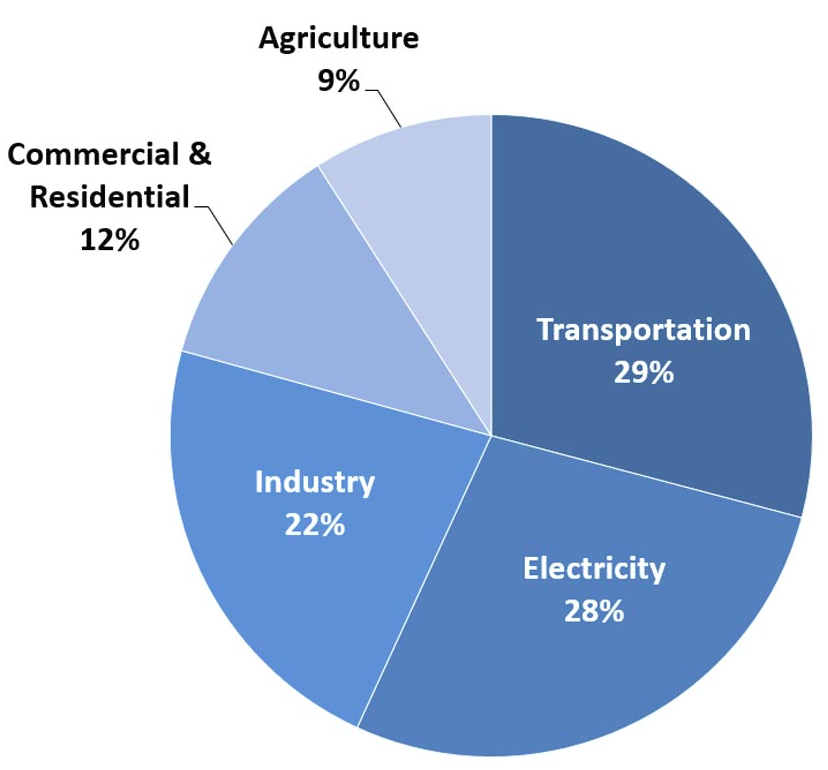
\includegraphics[height=6.2cm]{images/total-ghg-2017.png}
		\end{center}
		\caption{Total U.S. GHG Emissions by Economic Sector in 2017 \cite{us_epa_sources_2020}.}
	\end{figure}

	\column[t]{5cm}
	\begin{itemize}
		\item Illinois Climate Action Plan (iCAP).
		\item Attain carbon neutrality by 2050.
	\end{itemize}
\end{columns}
\end{frame}

% Notes:
% Transportation and Electricity are the economic sectors that produced ...

\begin{frame}
\frametitle{Transportation}
\begin{columns}
	\column[t]{5cm}
	\begin{itemize}
		\item Hydrogen economy
		\item california, japan, germany
	\end{itemize}

% Maybe a figure?
 %    \column[t]{5cm}
	% \begin{figure}[htbp!]
	% 	\begin{center}
	% 		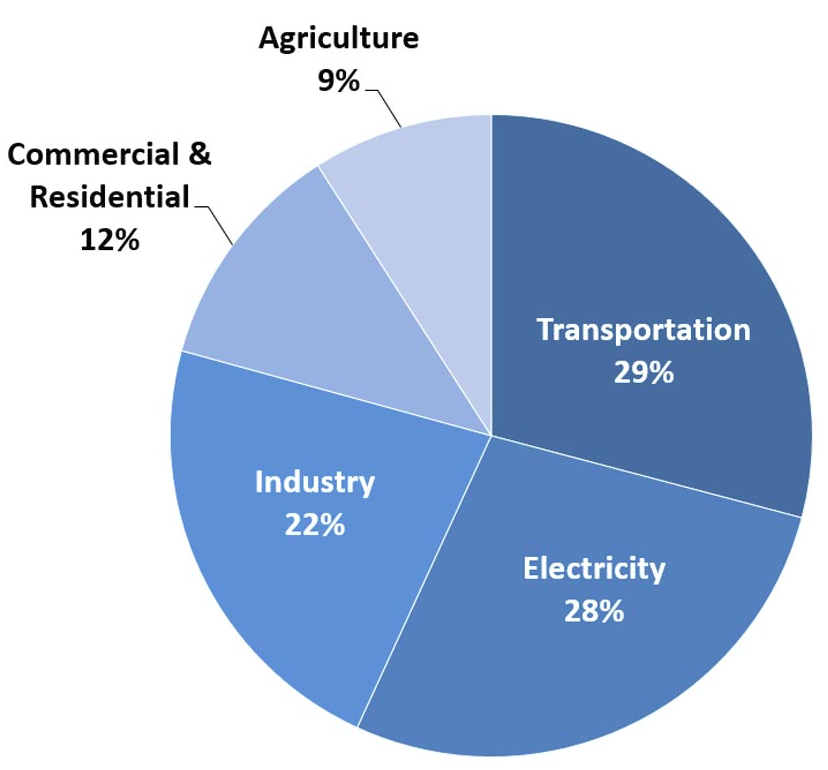
\includegraphics[height=6.2cm]{images/total-ghg-2017.png}
	% 	\end{center}
	% 	\caption{Total U.S. GHG Emissions by Economic Sector in 2017 \cite{us_epa_sources_2020}.}
	% \end{figure}
\end{columns}
\end{frame}

\begin{frame}
\frametitle{Electricity}
\begin{columns}
	\column[t]{5cm}
	\begin{itemize}
		\item More renewables
		\item Duck curve
	\end{itemize}

% Maybe a figure?
 %    \column[t]{5cm}
	% \begin{figure}[htbp!]
	% 	\begin{center}
	% 		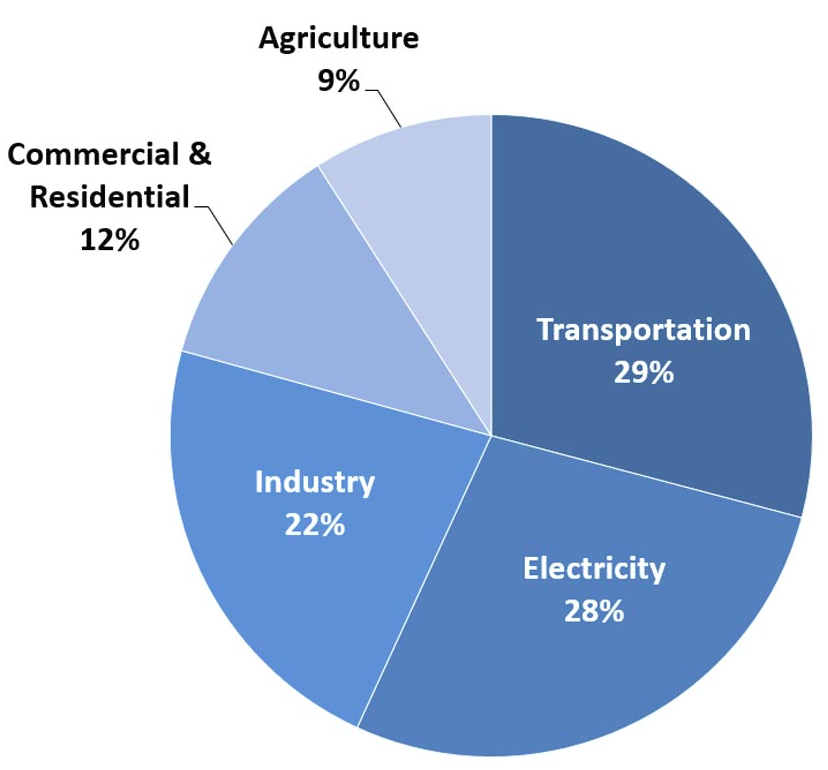
\includegraphics[height=6.2cm]{images/total-ghg-2017.png}
	% 	\end{center}
	% 	\caption{Total U.S. GHG Emissions by Economic Sector in 2017 \cite{us_epa_sources_2020}.}
	% \end{figure}
\end{columns}
\end{frame}

















% \begin{frame}
% \frametitle{"There must be something wrong at SL-1"}
% \begin{columns}
%     \column[t]{5cm}
% 	\begin{itemize}
% 		\item 9:01 pm alarm goes off at the main firehouse.
% 		\item Radiation readings too high, no signs of the crew.
% 		\item Ed Vallario went inside and saw Jack Byrnes.
% 		\item Retrieval of Byrnes and finding  of Legg.
% 		\item Byrnes was pronounced dead at 11:14 PM.
% 		\item Another group found the 3rd member pinned to the roof.
% 	\end{itemize}

%     \column[t]{5cm}
% 	\begin{itemize}
%         \item Retrieval of Legg's body.
%         \item Retrieval of McKinley's body.
%         \item Bodies taken to processing plant.
% 	\end{itemize}

%     "We got a reading on the detector, that by todays' standards, you'd have gotten the hell out of there." \textit{Lamprecht}.
%     \\
%     "I went to take a breath and it was like there was no more oxygen in the tank." \textit{Vallario}.

% \end{columns}
% \end{frame}

% \begin{frame}
% \frametitle{The accident}
% \begin{columns}
%     \column[t]{5cm}
% 	\begin{figure}[htbp!]
% 		\begin{center}
% 			\includegraphics[height=4.5cm]{./images/crew1a.png}
% 		\end{center}
% 		\caption{Reactor crew positions before the accident \cite{mckeown2003idaho}.}
% 	\end{figure}

%     \column[t]{5cm}
% 	\begin{itemize}
% 		\item Central rod is withdrawn 20".
% 		\item Reactor goes critical at 16.7".
% 		\item Fuel plates vaporize, water gets to 3740$^{\circ}$ F.
% 		\item Center fuel elements and central control blade ejected.
% 		\item Vessel rises out of its sheat and hits the ceiling.
% 		\item Vessel falls down.
% 	\end{itemize}
% \end{columns}
% \end{frame}


% \begin{frame}
% \frametitle{Theories}

% ”The direct cause of the incident clearly appears to have been the manual withdrawal by one or more of the maintenance crew of the central control rod blade from the SL-1 core considerably beyond the limit specified in the maintenance procedure. The reason or motive for the abnormal withdrawal is considered highly speculative, and it does not appear at all likely that there will ever be any reasons to change this judgment.”

% \end{frame}

% \begin{frame}
% \frametitle{Evaluation}
% 	\begin{block}{Author and Audience}
% 		\begin{itemize}
% 			\item Sources: Interviews and official documents.
% 			\item Wide audience.
% 		\end{itemize}
% 	\end{block}

% 	\begin{block}{Technical Evaluation}
% 		\begin{itemize}
% 			\item Technical explanation is not too extensive.
% 			\item A lot of details on the post-accident procedures.
% 			\item Description of the autopsies is extremely detailed.
% 		\end{itemize}
% 	\end{block}

% 	\begin{block}{Non-Technical Evaluation}
% 		\begin{itemize}
% 			\item Anecdotes, feelings, and opinions.
% 			\item Several theories on why Byrnes pulled from the rod.
% 			\item Verifiability is lost.
% 		\end{itemize}
% 	\end{block}
% \end{frame}

\section{Hydrogen Production Methods}
% \subsection{Hydrogen production methods}
\begin{frame}
\frametitle{Electrolysis}
\begin{columns}
    \column[t]{5cm}
	\begin{figure}[htbp!]
		\begin{center}
			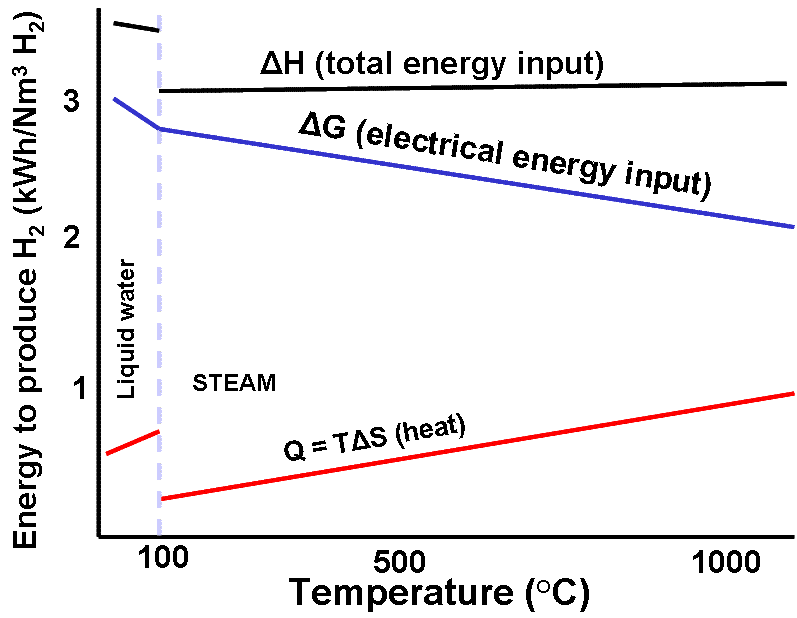
\includegraphics[height=4.0cm]{images/ele-curve.png}
		\end{center}
		\caption{Energy consumption of an ideal electrolysis process \cite{hi2h2_highly_2007}.}
	\end{figure}

	\column[t]{5cm}
	$\Delta$H: Required energy.
	\\
	$\Delta$G: Electrical energy.
	\\
	T$\Delta$S: Thermal energy. \vspace{0.7cm}

    In low temperature electrolysis (LTE), electricity provides the thermal energy.
    \\
    In high temperature electrolysis (HTE), heat source provides the thermal energy.
    \\
    HTE has the advantage of decreasing the electricity requirement.
    
\end{columns}
\end{frame}


\begin{frame}
\frametitle{Sulfur-Iodine}
\begin{columns}
    \column[t]{5cm}
   	\begin{figure}[htbp!]
		\begin{center}
			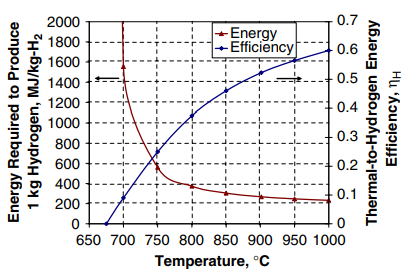
\includegraphics[height=4.0cm]{images/si-energy.png}
		\end{center}
		\caption{Sulfur-Iodine thermochemical cycle.}
 	\end{figure}

 	\column[t]{5cm}
 	\begin{itemize}
 		\item 3 different reactions: Sulfuric acid decomposition, Bunsen reaction, and hydrogen iodide decomposition.
 		\item Input: H$_2$O.
 		\item Output: H$_2$ $\&$ O$_2$. 
 		\item Does not require electricity.
 		\item Need of a high temperature source.
 	\end{itemize}
\end{columns}
\end{frame}

\subsection{Nuclear energy-based hydrogen}
\begin{frame}
\frametitle{Co-generation}
\begin{columns}
    \column[t]{6.5cm}
   	\begin{figure}[htbp!]
		\begin{center}
			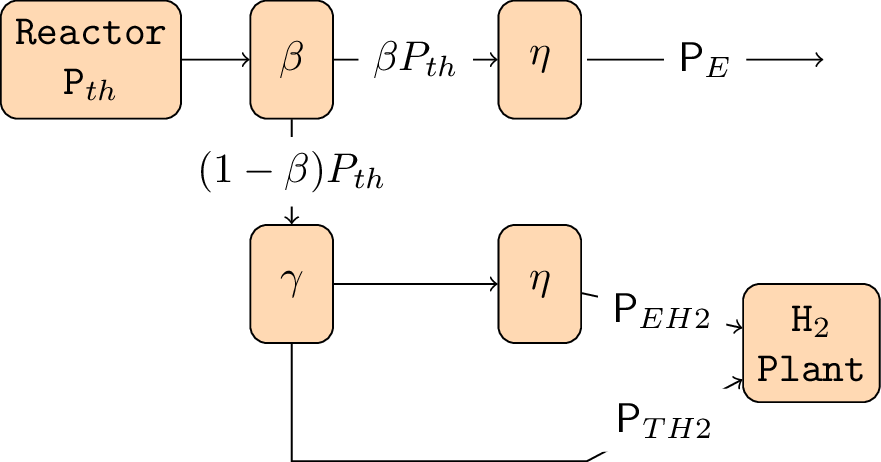
\includegraphics[height=3.6cm]{images/hte-figure0.png}
		\end{center}
		\caption{Reactor coupled to hydrogen plant diagram.}
 	\end{figure}

 	\column[t]{3.5cm}
 	$\beta$: power fraction that is converted into electricity.
 	\\
    $\beta$ = 1: no hydrogen is produced.
    \\
 	$\beta$ = 0: no electricity is produced. \vspace{0.6cm}

 	LTE:
 	\begin{itemize}
 		\item $\gamma$=1. P$_{TH2}$ = 0.
 	\end{itemize}

 	HTE:
 	\begin{itemize}
 		\item 0 $< \gamma <$ 1.
 	\end{itemize}

    SI:
 	\begin{itemize}
 		\item $\gamma$=0. P$_{EH2}$ = 0.
 	\end{itemize}


\end{columns}
\end{frame}

\section{Microreactors}
% \input{microreactors}

% \section{Future studies}
% \subsection{Hydrogen production methods}
\begin{frame}
\frametitle{Electrolysis}
\begin{columns}
    \column[t]{5cm}
	\begin{figure}[htbp!]
		\begin{center}
			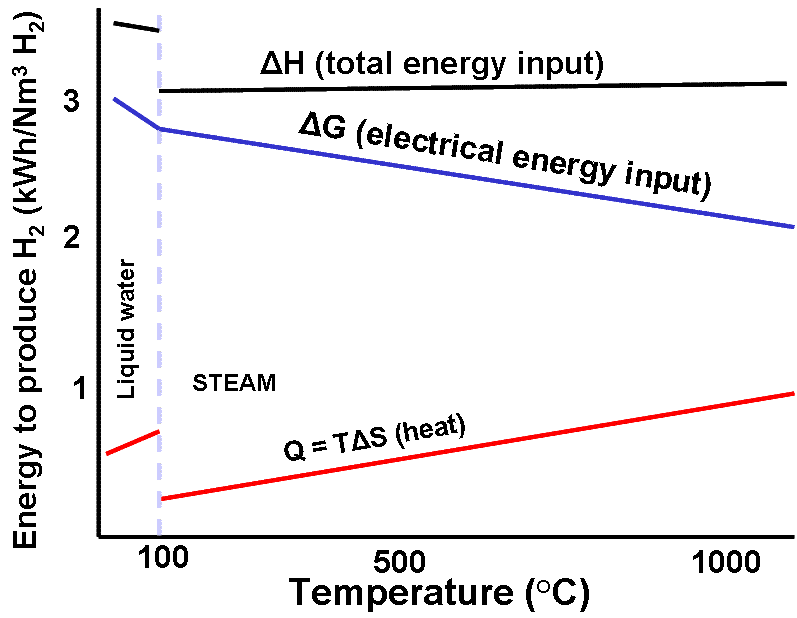
\includegraphics[height=4.0cm]{images/ele-curve.png}
		\end{center}
		\caption{Energy consumption of an ideal electrolysis process \cite{hi2h2_highly_2007}.}
	\end{figure}

	\column[t]{5cm}
	$\Delta$H: Required energy.
	\\
	$\Delta$G: Electrical energy.
	\\
	T$\Delta$S: Thermal energy. \vspace{0.7cm}

    In low temperature electrolysis (LTE), electricity provides the thermal energy.
    \\
    In high temperature electrolysis (HTE), heat source provides the thermal energy.
    \\
    HTE has the advantage of decreasing the electricity requirement.
    
\end{columns}
\end{frame}


\begin{frame}
\frametitle{Sulfur-Iodine}
\begin{columns}
    \column[t]{5cm}
   	\begin{figure}[htbp!]
		\begin{center}
			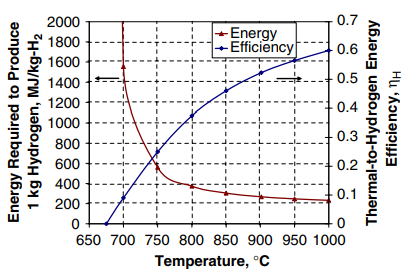
\includegraphics[height=4.0cm]{images/si-energy.png}
		\end{center}
		\caption{Sulfur-Iodine thermochemical cycle.}
 	\end{figure}

 	\column[t]{5cm}
 	\begin{itemize}
 		\item 3 different reactions: Sulfuric acid decomposition, Bunsen reaction, and hydrogen iodide decomposition.
 		\item Input: H$_2$O.
 		\item Output: H$_2$ $\&$ O$_2$. 
 		\item Does not require electricity.
 		\item Need of a high temperature source.
 	\end{itemize}
\end{columns}
\end{frame}

\subsection{Nuclear energy-based hydrogen}
\begin{frame}
\frametitle{Co-generation}
\begin{columns}
    \column[t]{6.5cm}
   	\begin{figure}[htbp!]
		\begin{center}
			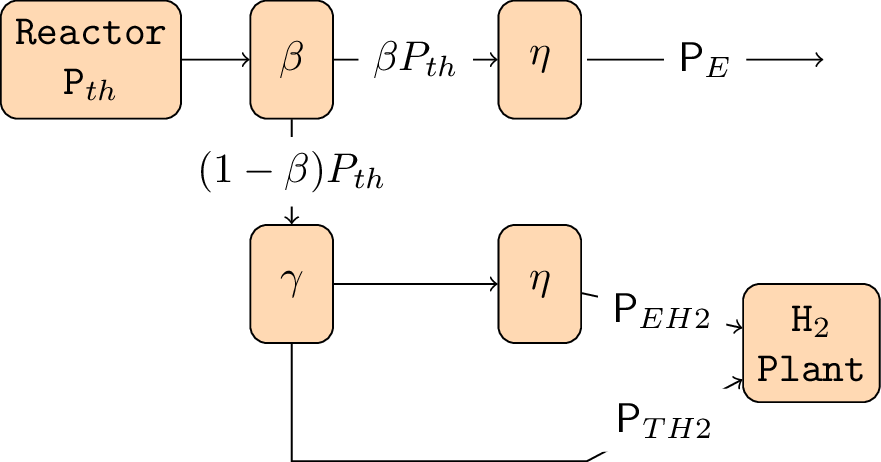
\includegraphics[height=3.6cm]{images/hte-figure0.png}
		\end{center}
		\caption{Reactor coupled to hydrogen plant diagram.}
 	\end{figure}

 	\column[t]{3.5cm}
 	$\beta$: power fraction that is converted into electricity.
 	\\
    $\beta$ = 1: no hydrogen is produced.
    \\
 	$\beta$ = 0: no electricity is produced. \vspace{0.6cm}

 	LTE:
 	\begin{itemize}
 		\item $\gamma$=1. P$_{TH2}$ = 0.
 	\end{itemize}

 	HTE:
 	\begin{itemize}
 		\item 0 $< \gamma <$ 1.
 	\end{itemize}

    SI:
 	\begin{itemize}
 		\item $\gamma$=0. P$_{EH2}$ = 0.
 	\end{itemize}


\end{columns}
\end{frame}

% \section{Conclusion}
% \begin{frame}
  \frametitle{Conclusion}
\end{frame}


\begin{frame}[allowframebreaks]
  \frametitle{References}
  \bibliographystyle{plain}
  {\footnotesize \bibliography{bibliography.bib} }
\end{frame}

\end{document}
